\documentclass[12pt]{beamer}\usepackage[]{graphicx}\usepackage[]{color}
%% maxwidth is the original width if it is less than linewidth
%% otherwise use linewidth (to make sure the graphics do not exceed the margin)
\makeatletter
\def\maxwidth{ %
  \ifdim\Gin@nat@width>\linewidth
    \linewidth
  \else
    \Gin@nat@width
  \fi
}
\makeatother

\definecolor{fgcolor}{rgb}{0.345, 0.345, 0.345}
\newcommand{\hlnum}[1]{\textcolor[rgb]{0.686,0.059,0.569}{#1}}%
\newcommand{\hlstr}[1]{\textcolor[rgb]{0.192,0.494,0.8}{#1}}%
\newcommand{\hlcom}[1]{\textcolor[rgb]{0.678,0.584,0.686}{\textit{#1}}}%
\newcommand{\hlopt}[1]{\textcolor[rgb]{0,0,0}{#1}}%
\newcommand{\hlstd}[1]{\textcolor[rgb]{0.345,0.345,0.345}{#1}}%
\newcommand{\hlkwa}[1]{\textcolor[rgb]{0.161,0.373,0.58}{\textbf{#1}}}%
\newcommand{\hlkwb}[1]{\textcolor[rgb]{0.69,0.353,0.396}{#1}}%
\newcommand{\hlkwc}[1]{\textcolor[rgb]{0.333,0.667,0.333}{#1}}%
\newcommand{\hlkwd}[1]{\textcolor[rgb]{0.737,0.353,0.396}{\textbf{#1}}}%
\let\hlipl\hlkwb

\usepackage{framed}
\makeatletter
\newenvironment{kframe}{%
 \def\at@end@of@kframe{}%
 \ifinner\ifhmode%
  \def\at@end@of@kframe{\end{minipage}}%
  \begin{minipage}{\columnwidth}%
 \fi\fi%
 \def\FrameCommand##1{\hskip\@totalleftmargin \hskip-\fboxsep
 \colorbox{shadecolor}{##1}\hskip-\fboxsep
     % There is no \\@totalrightmargin, so:
     \hskip-\linewidth \hskip-\@totalleftmargin \hskip\columnwidth}%
 \MakeFramed {\advance\hsize-\width
   \@totalleftmargin\z@ \linewidth\hsize
   \@setminipage}}%
 {\par\unskip\endMakeFramed%
 \at@end@of@kframe}
\makeatother

\definecolor{shadecolor}{rgb}{.97, .97, .97}
\definecolor{messagecolor}{rgb}{0, 0, 0}
\definecolor{warningcolor}{rgb}{1, 0, 1}
\definecolor{errorcolor}{rgb}{1, 0, 0}
\newenvironment{knitrout}{}{} % an empty environment to be redefined in TeX

\usepackage{alltt}
\usepackage{tikz}

% make it pretty
% get rid of junk
\usetheme{default}
\usefonttheme[onlymath]{serif}
\beamertemplatenavigationsymbolsempty

% define a bunch of colors
\definecolor{offwhite}{RGB}{255,250,240}
\definecolor{gray}{RGB}{155,155,155}
\definecolor{foreground}{RGB}{80,80,80}
\definecolor{background}{RGB}{255,255,255}
%\definecolor{title}{RGB}{255,199,0}
\definecolor{title}{RGB}{89,132,212}
%\definecolor{subtitle}{RGB}{89,132,212}
\definecolor{subtitle}{RGB}{255,199,0}
\definecolor{hilit}{RGB}{248,117,79}
\definecolor{vhilit}{RGB}{255,111,207}
\definecolor{lolit}{RGB}{200,200,200}
\definecolor{lit}{RGB}{255,199,0}
\definecolor{mdlit}{RGB}{89,132,212}
\definecolor{link}{RGB}{248,117,79}

% a few color macros
\newcommand{\hilit}{\color{hilit}}
\newcommand{\vhilit}{\color{vhilit}}
\newcommand{\lit}{\color{lit}}
\newcommand{\mdlit}{\color{mdlit}}
\newcommand{\lolit}{\color{lolit}}

% use those colors
\setbeamercolor{titlelike}{fg=title}
\setbeamercolor{subtitle}{fg=subtitle}
\setbeamercolor{frametitle}{fg=gray}
%\setbeamercolor{structure}{fg=subtitle}
\setbeamercolor{structure}{fg=title}
\setbeamercolor{institute}{fg=lolit}
\setbeamercolor{normal text}{fg=foreground,bg=background}
\setbeamertemplate{itemize subitem}{{\textendash}}
\setbeamerfont{itemize/enumerate subbody}{size=\small}
\setbeamerfont{itemize/enumerate subitem}{size=\small}

% center title of slides
\setbeamertemplate{blocks}[rounded]
\setbeamertemplate{frametitle}[default][center]

% page number
\setbeamerfont{page number in foot}{size=\footnotesize}
\setbeamertemplate{footline}[frame number]

% default link color
\hypersetup{colorlinks, urlcolor={link}}

% a few macros
\newcommand{\code}[1]{\texttt{#1}}
\newcommand{\hicode}[1]{{\hilit \texttt{#1}}}
\newcommand{\locode}[1]{{\lolit \texttt{#1}}}
\newcommand{\bb}[1]{\begin{block}{#1}}
\newcommand{\eb}{\end{block}}
\newcommand{\bi}{\begin{itemize}}
\newcommand{\bbi}{\vspace{4pt} \begin{itemize} \itemsep8pt}
\newcommand{\ei}{\end{itemize}}
\newcommand{\bv}{\begin{verbatim}}
\newcommand{\ev}{\end{verbatim}}
\newcommand{\ig}{\includegraphics}
\newcommand{\subt}[1]{{\footnotesize \color{subtitle} {#1}}}
\newcommand{\ttsm}{\tt \small}
\newcommand{\ttfn}{\tt \footnotesize}
\newcommand{\figh}[2]{\centerline{\includegraphics[height=#2\textheight]{#1}}}
\newcommand{\figw}[2]{\centerline{\includegraphics[width=#2\textwidth]{#1}}}



%------------------------------------------------

\title{Classic Examples}
\subtitle{Intro to Data Visualization}
\author{\href{http://www.gastonsanchez.com}{Gaston Sanchez}}
\institute{\href{https://creativecommons.org/licenses/by-sa/4.0/}{\tt \scriptsize \color{foreground} CC BY-SA 4.0}}
\date{}
\IfFileExists{upquote.sty}{\usepackage{upquote}}{}
\begin{document}



% no page number in first slide
{
  \setbeamertemplate{footline}{} 
  \frame{\titlepage} 
}

%------------------------------------------------

\begin{frame}
\begin{center}
\Huge{\hilit{Minard's Map}}
\end{center}
\end{frame}

%------------------------------------------------

\begin{frame}
\frametitle{}
\begin{center}
\ig[height=7cm]{images/napoleon.jpg}

{\tiny {\lolit \textit{Napoleon crossing the Alps} by Jacques Louis David.
(The horse is beleived to be Marengo)}}
\end{center}
\end{frame}

%------------------------------------------------

{ % all template changes are local to this group.
    \begin{frame}[plain]
        \begin{tikzpicture}[remember picture,overlay]
            \node[at=(current page.center)] {
                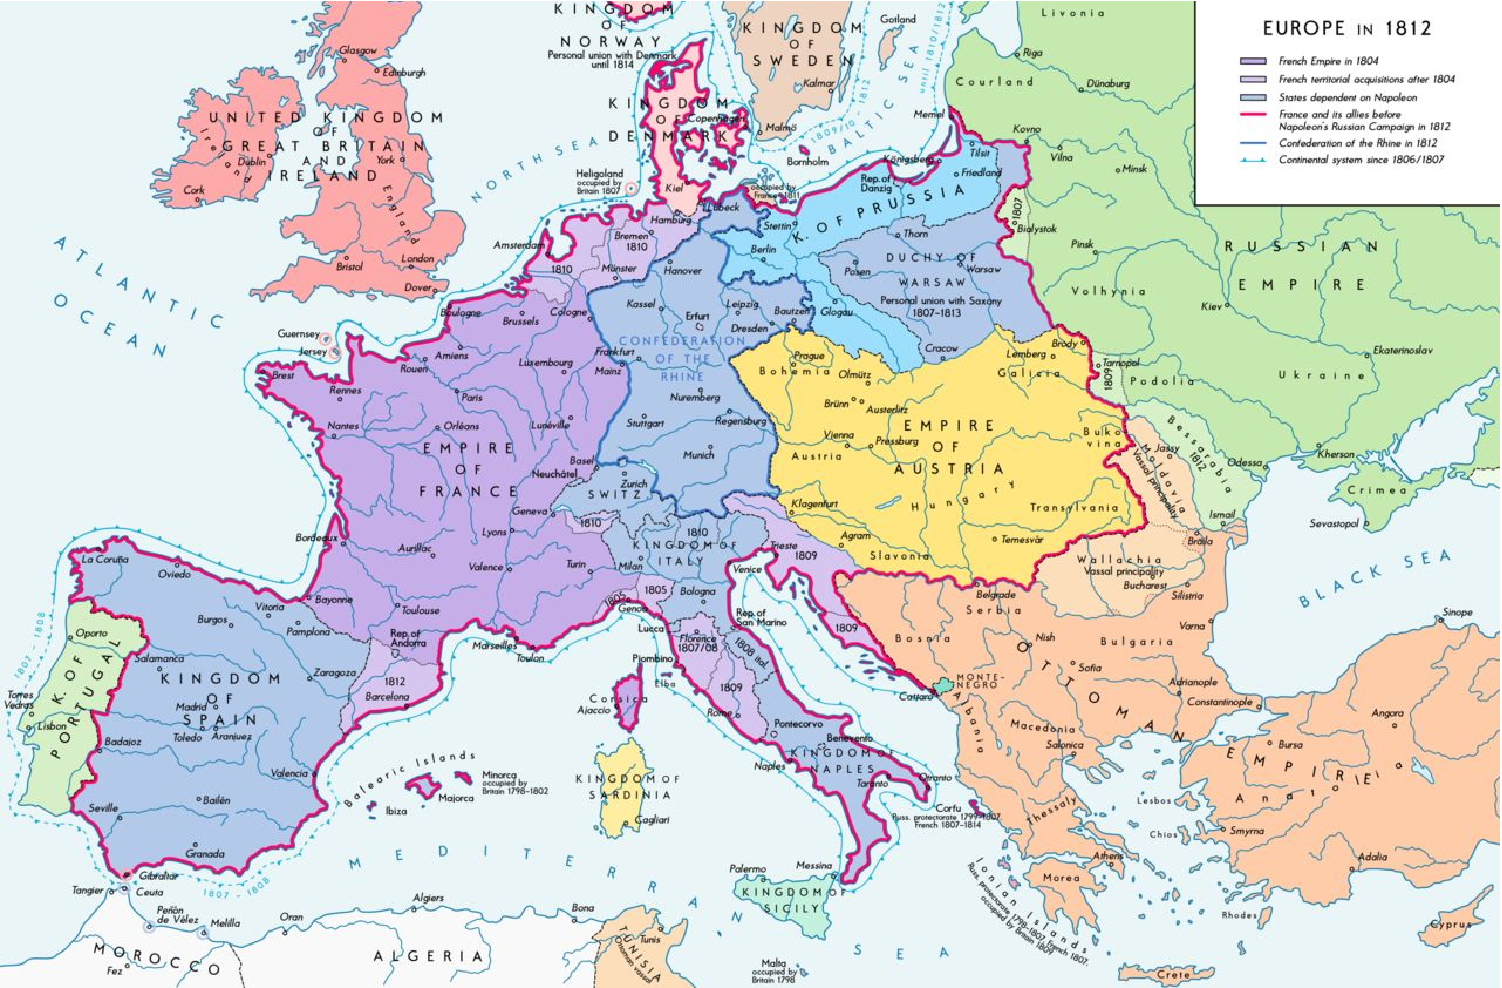
\includegraphics[width=\paperwidth]{images/europe-map-1812.pdf}
            };
        \end{tikzpicture}
     \end{frame}
}

%------------------------------------------------

\begin{frame}
\frametitle{Some historical background}

\bi
  \item \code{1776}: Declaration of independence (USA) 
  \item \code{1786}: French Revolution
  \item \code{1792}: French First Republic
  \item \code{1804}: French First Empire (Napoleon becomes emperor)
  \item \code{1803-1815}: Napoleonic Wars
  \item \code{1812}: War between US and United Kingdom
\ei

\end{frame}

%------------------------------------------------

\begin{frame}
\frametitle{Some historical background}

{\Large French Invasion of Russia}

\vspace{1cm}

{\Large \lit{June 1812}}

\vspace{1cm}

{\Large \hilit{Grand Armee (500,000 aprox)}}

{\tiny \url{https://en.wikipedia.org/wiki/French_invasion_of_Russia}}

\end{frame}

%------------------------------------------------

\begin{frame}
\frametitle{C.J. Minard}

\begin{columns}[t]
\begin{column}{0.4\textwidth}
\begin{center}
\ig[height=6cm]{images/charles-minard.pdf}
\end{center}
\end{column}

\begin{column}{0.5\textwidth}
\begin{center}
\bi
  \item Charles Joseph Minard (1781 - 1870)
  \item French Civil Engineer
  \item Created very novel and sophisticated graphics
\ei
\end{center}
\end{column}
\end{columns}

\begin{center}
{\tiny \url{https://en.wikipedia.org/wiki/Charles_Joseph_Minard}}
\end{center}

\end{frame}

%------------------------------------------------

{ % all template changes are local to this group.
    \begin{frame}[plain]
        \begin{tikzpicture}[remember picture,overlay]
            \node[at=(current page.center)] {
                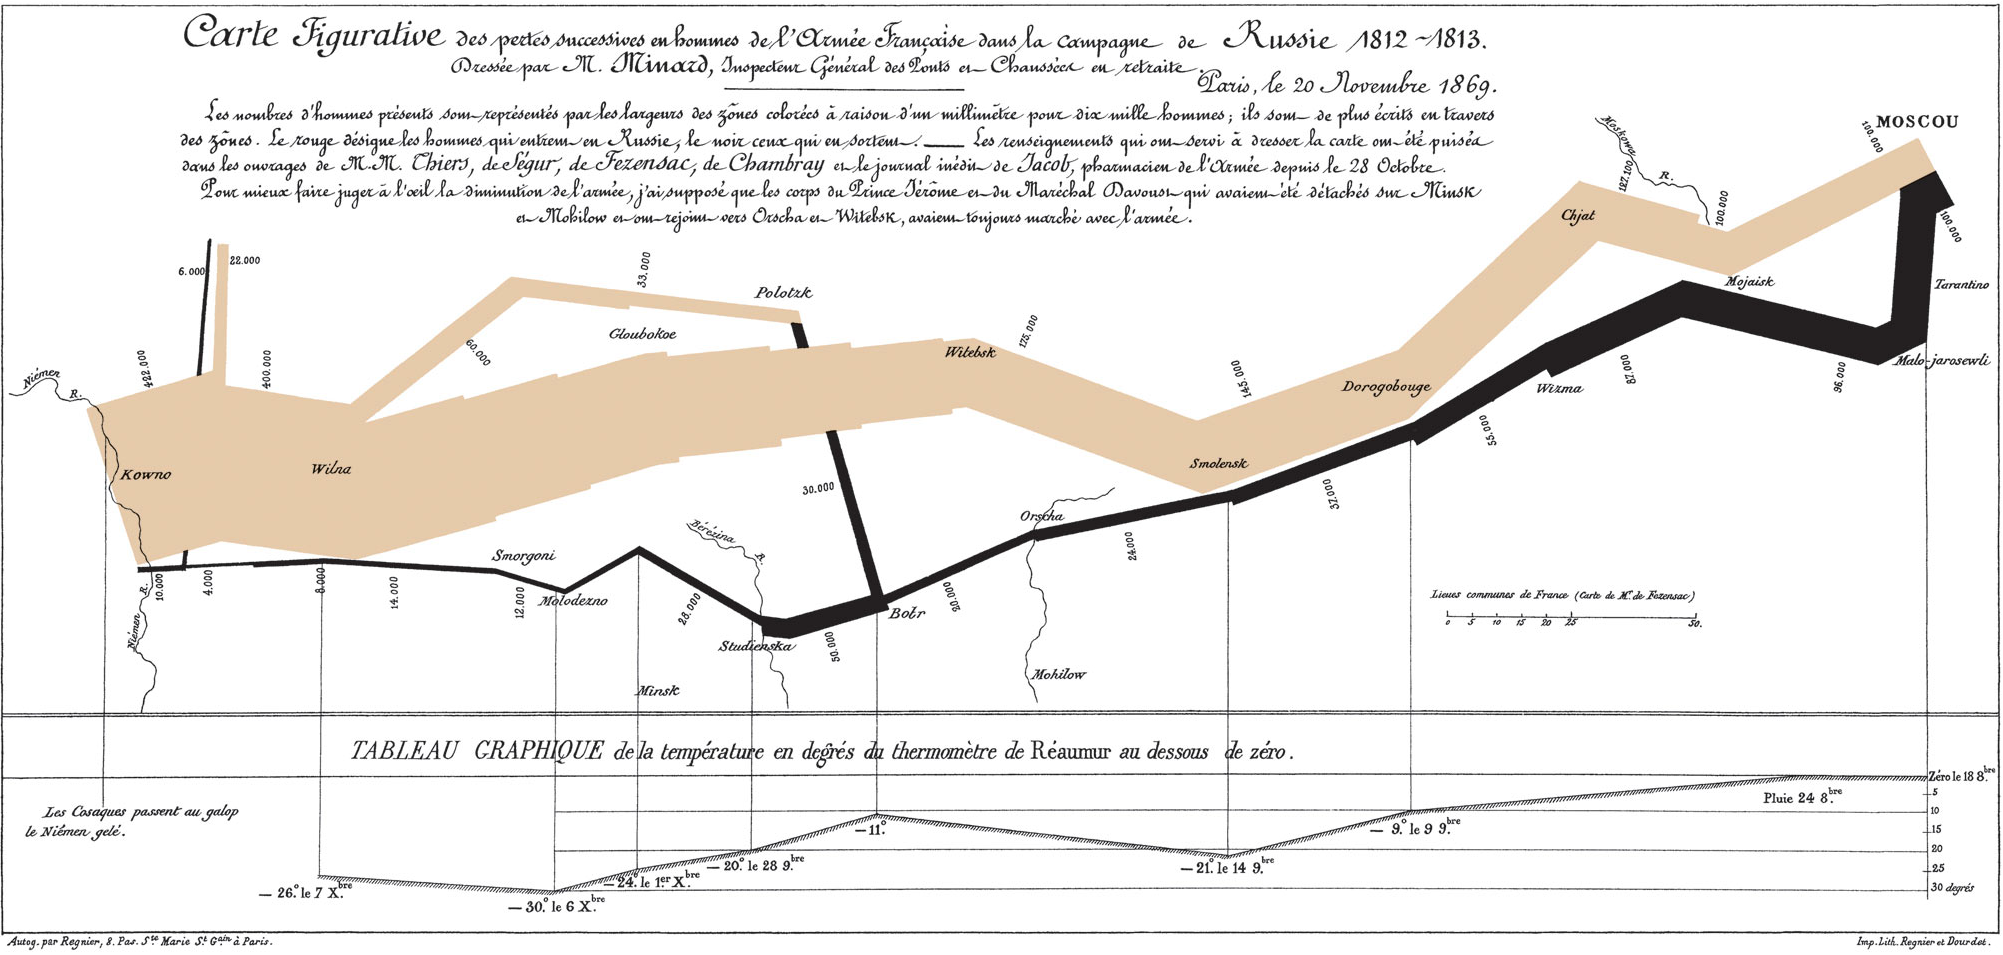
\includegraphics[width=\paperwidth]{images/minard-map.png}
            };
        \end{tikzpicture}
     \end{frame}
}

%------------------------------------------------

\begin{frame}
\frametitle{About Minard's map}

\bb{Seven variables in one chart}
\bi
  \item number of troops
  \item traveled distance
  \item temperature
  \item latitude
  \item longitude
  \item direction of travel
  \item location relative to specific dates
\ei
\eb

\end{frame}

%------------------------------------------------

{ % all template changes are local to this group.
    \begin{frame}[plain]
        \begin{tikzpicture}[remember picture,overlay]
            \node[at=(current page.center)] {
                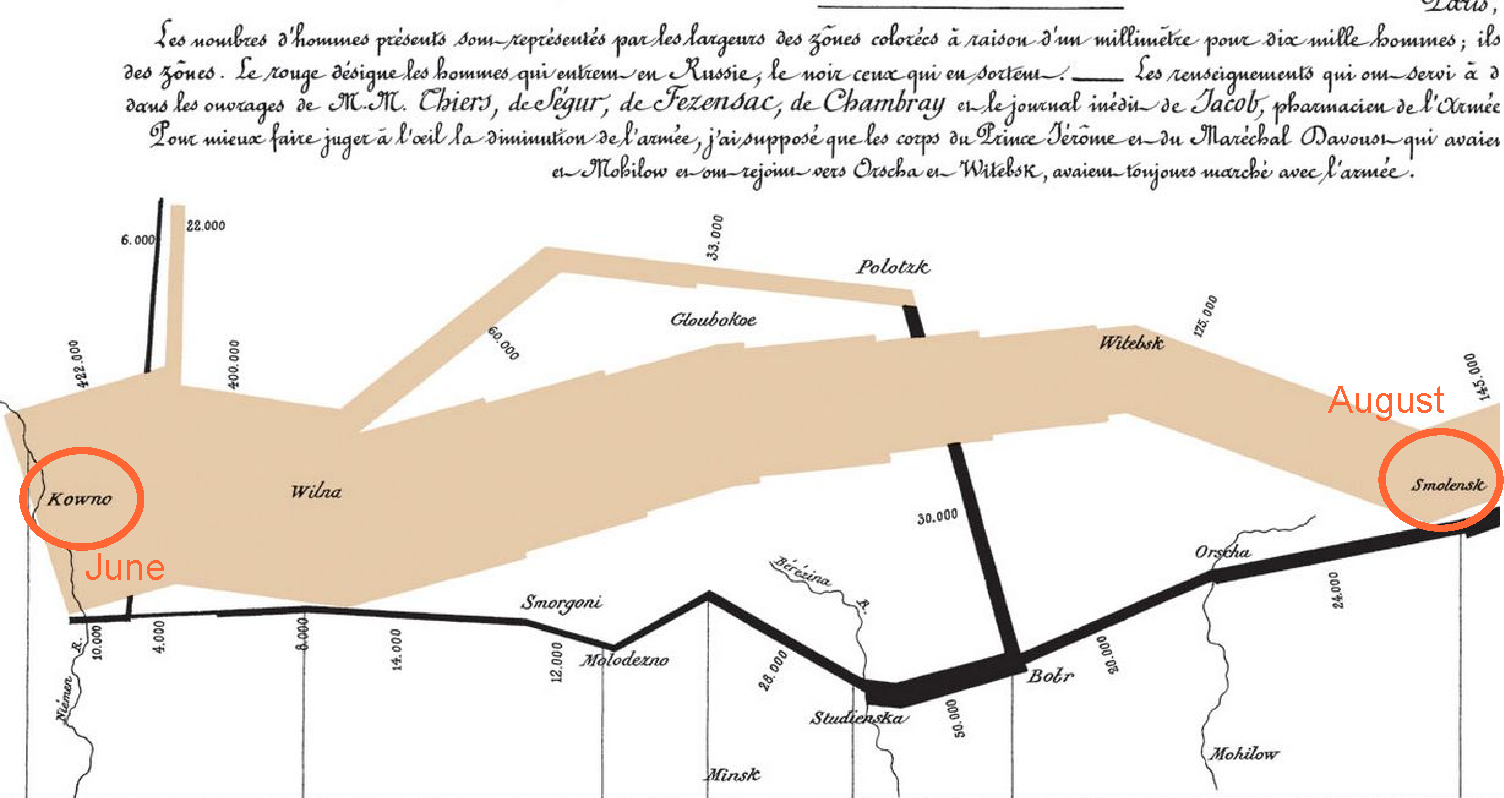
\includegraphics[width=\paperwidth]{images/kowno-smolensk-map.pdf}
            };
        \end{tikzpicture}
     \end{frame}
}

%------------------------------------------------

\begin{frame}
\frametitle{Russian Field Marshal Mikhail Kutuzov}
\begin{center}
\ig[width=11cm]{images/russian-generals.pdf}
\end{center}
\end{frame}

%------------------------------------------------

{ % all template changes are local to this group.
    \begin{frame}[plain]
        \begin{tikzpicture}[remember picture,overlay]
            \node[at=(current page.center)] {
                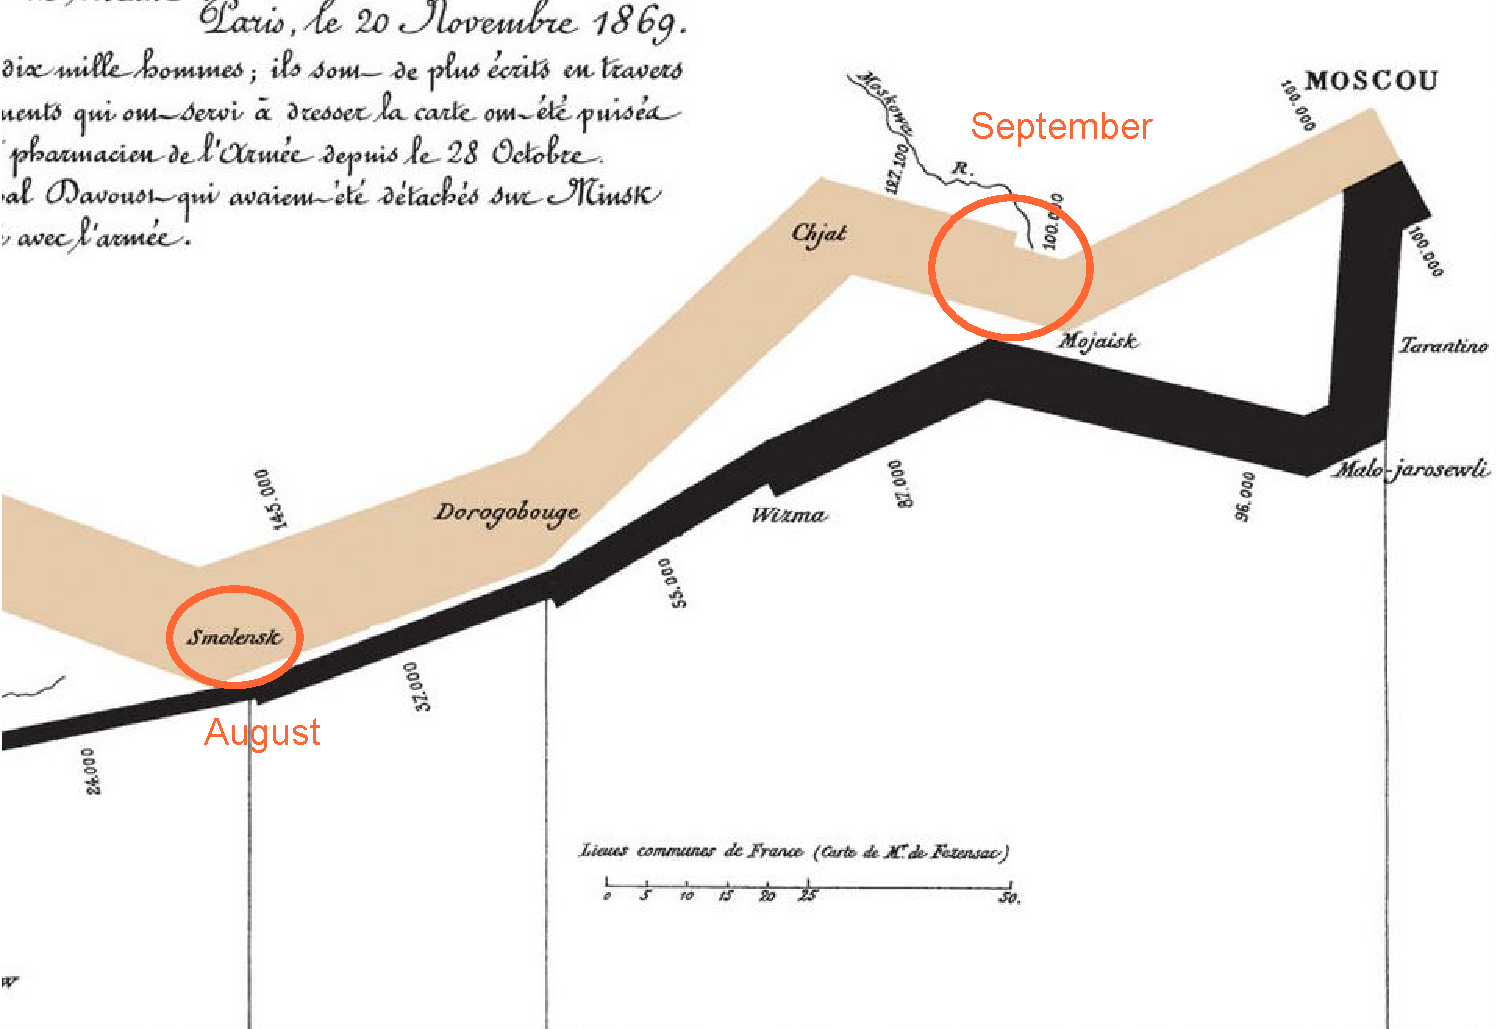
\includegraphics[width=\paperwidth]{images/smolensk-moscou-map.pdf}
            };
        \end{tikzpicture}
     \end{frame}
}

%------------------------------------------------

\begin{frame}
\frametitle{}
\begin{center}
\ig[height=8cm]{images/semyonov.jpg}

{\tiny {\lolit \textit{The Russian Army and residents of Moscow abandon the city in 1812}, by A. Semyonov and A. Sokolov.}}
\end{center}
\end{frame}

%------------------------------------------------

\begin{frame}
\frametitle{Some historical background}

{\Large Capture of Moscow}

\vspace{1cm}

{\Large \lit{September 1812}}

\vspace{1cm}

{\Large \hilit{(not so) Grand Armee (100,000 aprox)}}

\end{frame}

%------------------------------------------------

\begin{frame}
\frametitle{}
\begin{center}
\ig[width=11cm]{images/moscou-map.pdf}
\end{center}
\end{frame}

%------------------------------------------------

\begin{frame}
\frametitle{}
\begin{center}
\ig[width=10cm]{images/napoleons-retreat.pdf}

{\tiny {\lolit \textit{Napoleon's retreat from Moscow}, by Viktor Mazurovsky.}}
\end{center}
\end{frame}

%------------------------------------------------

{ % all template changes are local to this group.
    \begin{frame}[plain]
        \begin{tikzpicture}[remember picture,overlay]
            \node[at=(current page.center)] {
                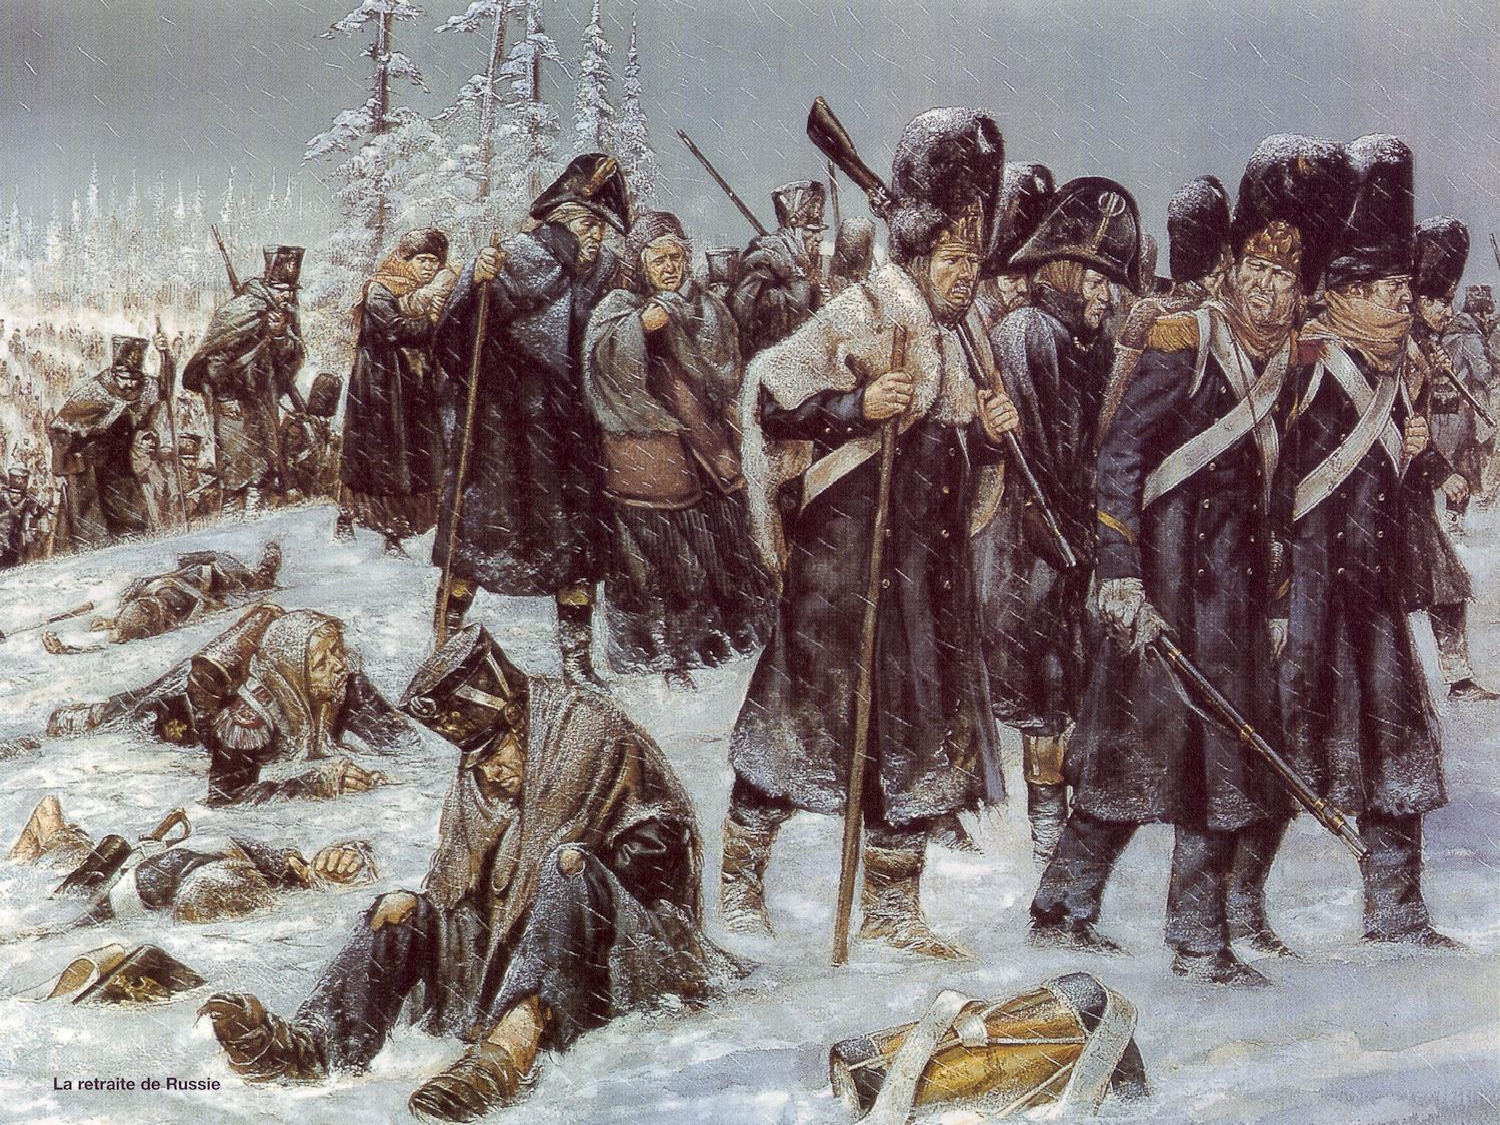
\includegraphics[width=\paperwidth]{images/retraite-russie.pdf}
            };
        \end{tikzpicture}
     \end{frame}
}

%------------------------------------------------

\begin{frame}
\frametitle{}
\begin{center}
\ig[width=11cm]{images/10000-men.pdf}
\end{center}
\end{frame}

%------------------------------------------------

\begin{frame}
\begin{center}
\Huge{\hilit{Challenger Explosion (1986)}}
\end{center}
\end{frame}

%------------------------------------------------

{ % all template changes are local to this group.
    \begin{frame}[plain]
        \begin{tikzpicture}[remember picture,overlay]
            \node[at=(current page.center)] {
                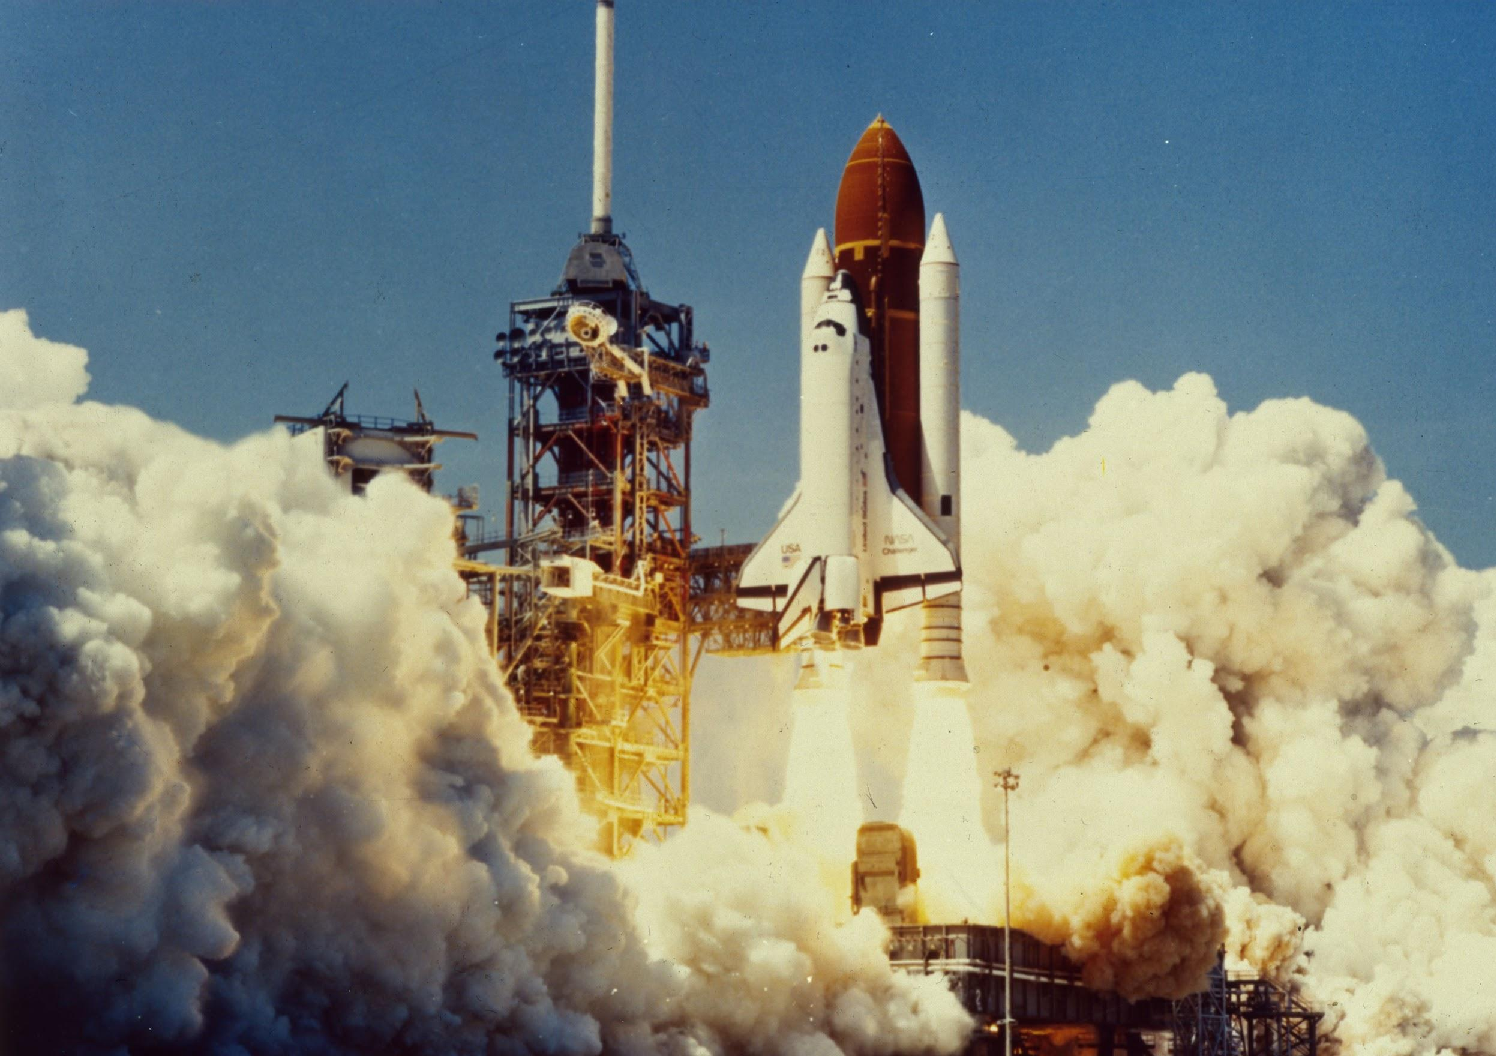
\includegraphics[width=\paperwidth]{images/challenger.pdf}
            };
        \end{tikzpicture}
     \end{frame}
}

%------------------------------------------------

\begin{frame}
\frametitle{A bit of context}

\bb{Some Remarks}
\bi
  \item Space Race
  \item Cold War (USA -vs- URSS)
  \item Many launching delays
  \item First civilian as part of the crew
  \item Reagan's ``State of the Union'' \\
  {\lolit planned the same day}
\ei
\eb

\end{frame}

%------------------------------------------------

\begin{frame}
\frametitle{}
\begin{center}
\ig[height=8cm]{images/major-malfunction-diagram.jpg}

{\tiny \url{https://www.awesomestories.com/asset/view/Challenger-and-the-Major-Malfunction//1}}
\end{center}
\end{frame}

%------------------------------------------------

{ % all template changes are local to this group.
    \begin{frame}[plain]
        \begin{tikzpicture}[remember picture,overlay]
            \node[at=(current page.center)] {
                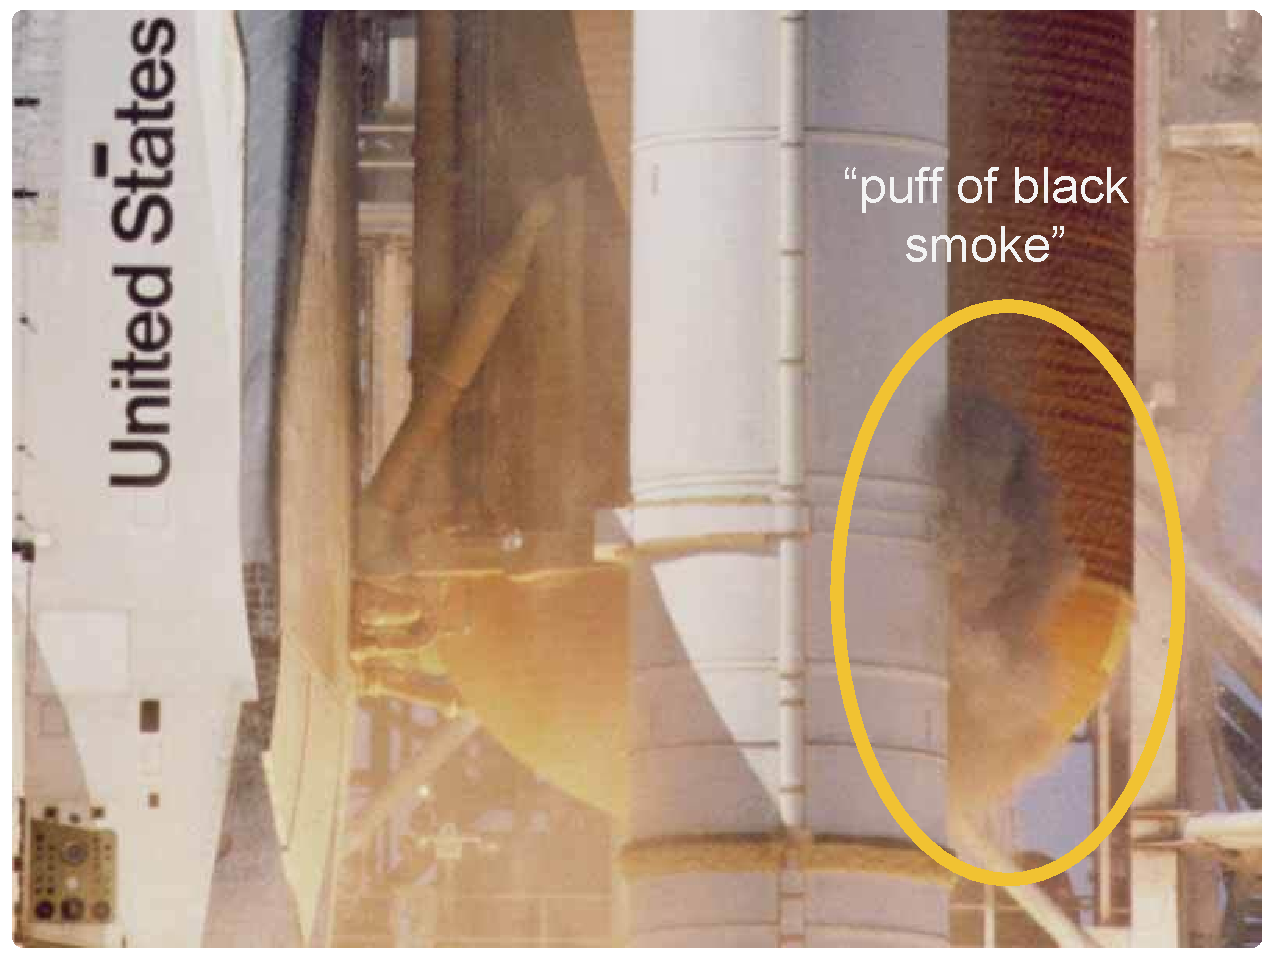
\includegraphics[width=\paperwidth]{images/challenger-smoke.pdf}
            };
        \end{tikzpicture}
     \end{frame}
}

%------------------------------------------------

\begin{frame}
\frametitle{}
\begin{center}
\ig[height=7cm]{images/roger-boisjoly.pdf}

{\scriptsize \lolit{Roger Boisjoly, c. 1991 (former Morton-Thiokol engineer)}}
\end{center}
\end{frame}

%------------------------------------------------

\begin{frame}
\frametitle{}
\begin{center}
\ig[height=7cm]{images/bob-ebeling.pdf}

{\scriptsize \lolit{Bob Ebeling, c. 2016 (former Morton-Thiokol engineer)}}
\end{center}
\end{frame}

%------------------------------------------------

\begin{frame}
\frametitle{}
\begin{center}
\ig[width=10cm]{images/oring-temp-incidents.pdf}

{\scriptsize \lolit{(24 launches with affected O-rings prior to the Challenger)}}
\end{center}
\end{frame}

%------------------------------------------------

\begin{frame}
\frametitle{}
\begin{center}
\ig[width=10cm]{images/oring-temp-damage.pdf}

{\scriptsize \lolit{(Published in shuttle commission report; unknown date of creation)}}
\end{center}
\end{frame}

%------------------------------------------------

\begin{frame}
\frametitle{}
\begin{center}
\ig[height=8cm]{images/challenger-incidents-table.pdf}

{\scriptsize \lolit{(based on Tufte)}}
\end{center}
\end{frame}

%------------------------------------------------

\begin{frame}
\frametitle{Some Remarks}

\bbi
  \item 13 charts were prepared for making the decision to launch
  \item 6 charts contained no tabled data about either O-ring temp, blow-by, or damage.
  \item The rest of charts contained no info about relation between temp and O-ring anomalies
  \item They all failed to reveal the risks of launching at very low temperatures
\ei

\end{frame}

%------------------------------------------------

\begin{frame}
\frametitle{}
\begin{center}
\ig[width=11cm]{images/oring-damage-scatter-plot1.pdf}
\end{center}
\end{frame}

%------------------------------------------------

\begin{frame}
\frametitle{}
\begin{center}
\ig[width=11cm]{images/oring-damage-scatter-plot2.pdf}
\end{center}
\end{frame}

%------------------------------------------------

\begin{frame}
\frametitle{}
\begin{center}
\ig[width=11cm]{images/oring-damage-scatter-plot3.pdf}
\end{center}
\end{frame}

%------------------------------------------------

\begin{frame}
\frametitle{Some resources}

\bi
  \item Space Shuttle Challenger Accident \\
  {\tiny \url{https://www.youtube.com/watch?v=fSTrmJtHLFU}}
  \item Inside Space Shuttle Challenger STS-51L During The Accident \\
  {\tiny \url{https://www.youtube.com/watch?v=NnmSdVbgQ4M}}
  \item NPR article about Bob Ebeling \\
  {\tiny \url{http://www.npr.org/sections/thetwo-way/2016/01/28/464744781/30-years-after-disaster-challenger-engineer-still-blames-himself}}
  \item Challenger Engineer Who Warned Of Shuttle Disaster Dies \\
  {\tiny \url{http://www.npr.org/sections/thetwo-way/2016/03/21/470870426/challenger-engineer-who-warned-of-shuttle-disaster-dies}}
\ei

\end{frame}

%------------------------------------------------

\begin{frame}
\begin{center}
\Huge{\hilit{Hans Rosling's Talks}}
\end{center}
\end{frame}

%------------------------------------------------

\begin{frame}
\frametitle{Communicate: Hans Rosling}
\begin{center}
\ig[width=10cm]{images/hans-rosling.pdf}
\end{center}
\end{frame}

%------------------------------------------------

\begin{frame}
\begin{center}
\large{\mdlit{Watch any (or better: all) of Hans Rosling videos and TED talks}}
\end{center}
\end{frame}

%------------------------------------------------

\begin{frame}
\frametitle{Hans Rosling}
\begin{center}
\ig[width=11cm]{images/hans-rosling-talks.pdf}
\end{center}
\end{frame}

%------------------------------------------------


\end{document}
